\documentclass{article}
\usepackage{graphicx} % Required for inserting images
\usepackage[spanish]{babel}
\usepackage{booktabs}

\title{Emisión de $CO_2$ de vehículos que circulan en México en base a sus características}
\author{Luis Felipe Rangel Salazar}
\date{Julio 2024}

\begin{document}

\maketitle

\section{Introducción}

El conjunto de datos con el que se va a trabajar representa un listado de distintos vehículos que circulan en México junto con sus características.

El objetivo del trabajo es identificar las principales características de un vehículo que afectan en su cantidad de emisiones de $CO_2$.

Se pretende hacer un análisis predictivo del nivel de contaminante que emiten los vehículos en base a algunas de sus características, y por consecuencia en la cantidad de dióxido de carbono ($CO_2$) que emiten, aplicando algunos métodos de Aprendizaje Supervisado o No Supervisado.



\section{Descripción de los datos}

La base de datos consta de 4,601 registros con 19 variables originalmente.

\begin{itemize}
    \item CO2 (g/km) [variable objetivo]
    \item Marca
    \item Submarca
    \item Versión
    \item Modelo
    \item Trans.
    \item Comb.
    \item Cilindros
    \item Categoría
    \item R. Ciudad (km/l)
    \item R. Carr. (km/l)
    \item R. Comb. (km/l)
    \item R. Ajust. (km/l)
    \item Nox (g/1000km)
    \item Calificación Gas Ef. Inv.
    \item Calificación Contam. Aire
    \item Tamaño (L)
    \item Potencia (HP)
    \item Hibrido 
\end{itemize}

\subsection{Selección de variables}

Las siguientes variables fueron descartadas:

\begin{itemize}
    \item R. Comb. (km/l)
    \item R. Ajust. (km/l)
    \item Nox (g/1000km)
    \item Calificación Gas Ef. Inv.
    \item Calificación Contam. Aire
    \item Versión
    \item Comb.
\end{itemize}

Esto, debido a que estas variables se derivan o se calculan en base a otras que ya estamos considerando, tales como R. Ciudad (km/l) y R. Carr. (km/l), con lo que si las incluimos tendríamos un problema de colinealidad. En el caso de Nox (g/1000km) y Comb. se excluyen por tener un bajo estadístico F en relación al CO2 (g/km). La variable Versión también debe ser excluida debido a que hay muchas categorías de Versión (3,118 etiquetas de 4,601 registros), esta variable no permite un análisis al casi tener cada vehículo su propia Versión.

Con esto se corre el riesgo de tener overfitting y por lo tanto la sugerencia es remover este campo.


\subsection{Estadística descriptiva básica}


A continuación se presenta la matriz de correlaciones entre las variables.

\begin{figure}[h]
  \centering
  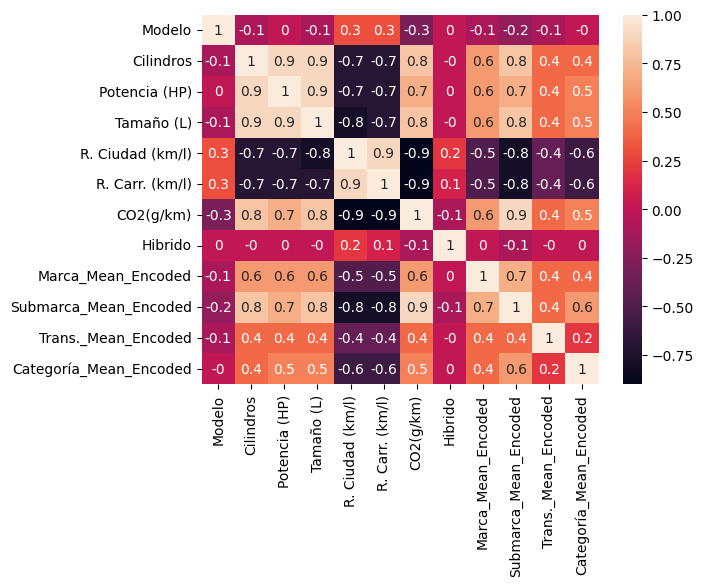
\includegraphics[width=1\linewidth]{imagenes/1_correlations.png}
  \caption{Matriz de correlaciones}
  \label{fig:nombre}
\end{figure}

Como se puede ver en la figuar 1, las variables de Cilindros, Potencia y Tamaño son las que se encuentran más correlacionadas positivamente entre ellas. De igual forma, la variable Submarca tiene una correalación positiva alta con la variable respuesta $CO_2$. Las variables de Rendimiento en Ciudad y Rendimiento en Carretera son las que presentan mayor correlación negativa con la variable respuesta $CO_2$.

Abajo se muestran las principales estadísticas descriptivas de cada variable.

\begin{tabular}{lrrrrr}
\toprule
 & Modelo & Cilindros & Potencia (HP) & Tamaño (L)\\
\midrule
Conteo & 4601.000000 & 4601.000000 & 4601.000000 & 4601.000000\\
Media & 2014.180000 & 5.330000 & 255.290000 & 2.870000\\
Desviación & 2.160000 & 1.800000 & 132.920000 & 1.350000\\
Min & 2011.000000 & 3.000000 & 60.000000 & 0.900000\\
25\% & 2012.000000 & 4.000000 & 150.000000 & 1.800000\\
50\% & 2014.000000 & 4.000000 & 220.000000 & 2.500000\\
75\% & 2016.000000 & 6.000000 & 330.000000 & 3.600000\\
Max & 2018.000000 & 12.000000 & 888.000000 & 8.400000\\
\bottomrule
\end{tabular}

\begin{tabular}{lrrrr}
\toprule
 & R. Ciudad (km/l) & R. Carr. (km/l) & CO2(g/km) & Hibrido \\
\midrule
Conteo & 4601.000000 & 4601.000000 & 4601.000000 & 4601.000000 \\
Media & 10.600000 & 16.600000 & 256.730000 & 0.010000 \\
Desviación & 3.290000 & 4.190000 & 75.630000 & 0.100000 \\
Min & 3.100000 & 6.700000 & 107.000000 & 0.000000 \\
25\% & 8.200000 & 13.440000 & 200.000000 & 0.000000 \\
50\% & 10.420000 & 16.390000 & 244.000000 & 0.000000 \\
75\% & 12.820000 & 19.600000 & 299.000000 & 0.000000 \\
Max & 27.460000 & 31.300000 & 627.000000 & 1.000000 \\
\bottomrule
\end{tabular}

\section{Preprocesamiento}

Se generó el campo Hibrido con un 1 si el vehículo es híbrido y 0 si no lo es, en base a la descripción del vehículo que se podía extraer de los campos Versión y Submarca. Se eliminaron los registros con valores nulos y se redefinieron las variables categóricas usando el método de Mean Encoding.


\section{Agrupamiento}

Se realizó un agrupamiento para la variable Submarca con $CO_2$ por el método de K-Medias.

Primero se obtuvo que la cantidad de grupos adecuada era $K=4$ de acuerdo al gráfico de codo.

\begin{figure}[h]
  \centering
  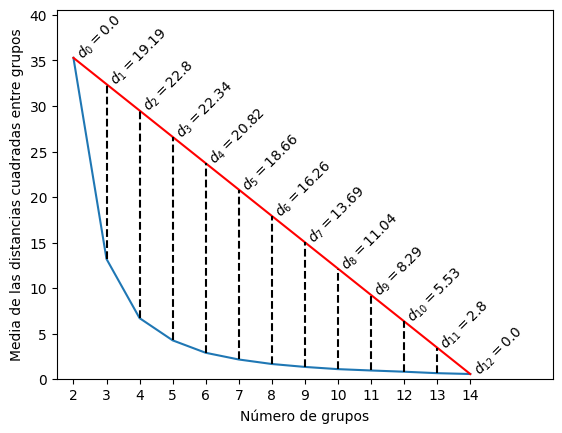
\includegraphics[width=.7\linewidth]{imagenes/2_codo.png}
  \caption{Gráfica de codo}
  \label{fig:nombre}
\end{figure}

\newpage

El resultado de emplear K-medias para agrupar las submarcas se puede apreciar en la figura 3.

\begin{figure}[h]
  \centering
  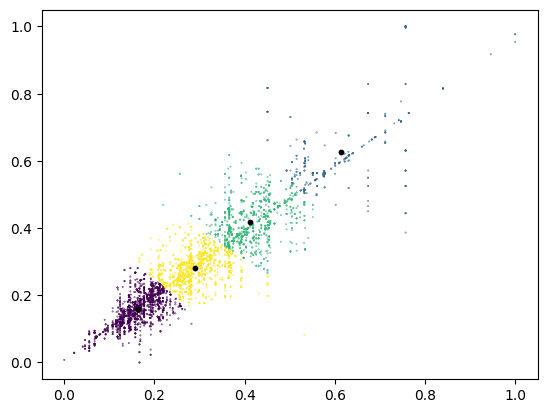
\includegraphics[width=.65\linewidth]{imagenes/3_k-medias.png}
  \caption{Gráfica de codo}
  \label{fig:nombre}
\end{figure}

\newpage

\bibliographystyle{unsrtnat}
\bibliography{biblio}

Información sobre las tendencias de emisiones de CO2 y rendimiento de combustible en Estados Unidos (en inglés):
EPA. (2016). Light-Duty Automotive Technology, Carbon Dioxide Emissions, and Fuel Economy Trends: 1975 Through 2016, United States Environmental Protection Agency (EPA).

Información sobre las tendencias mundiales de emisiones de gases de efecto mundiales provenientes de vehículos de pasajeros y rendimiento de combustible (en inglés):
An, F., Gordon, D., He, H., Kodjak, D., \& Rutherford, D. (2007). Passenger Vehicle Greenhouse Gas and Fuel Economy Standards: A Global Update, The InternationalCouncil on Clean Transportation (ICCT).

Información sobre las diferencias que existen entre el rendimiento ajustado por la EPA y el rendimiento observado consultar el documento (en inglés):
Greene, D., Goeltz, R., Hopson J. (2005). Analysis of In-Use Fuel Economy Shorfall by Means of Voluntarily Reported Fuel Economy Estimates.


\end{document}
